{
\usebackgroundtemplate{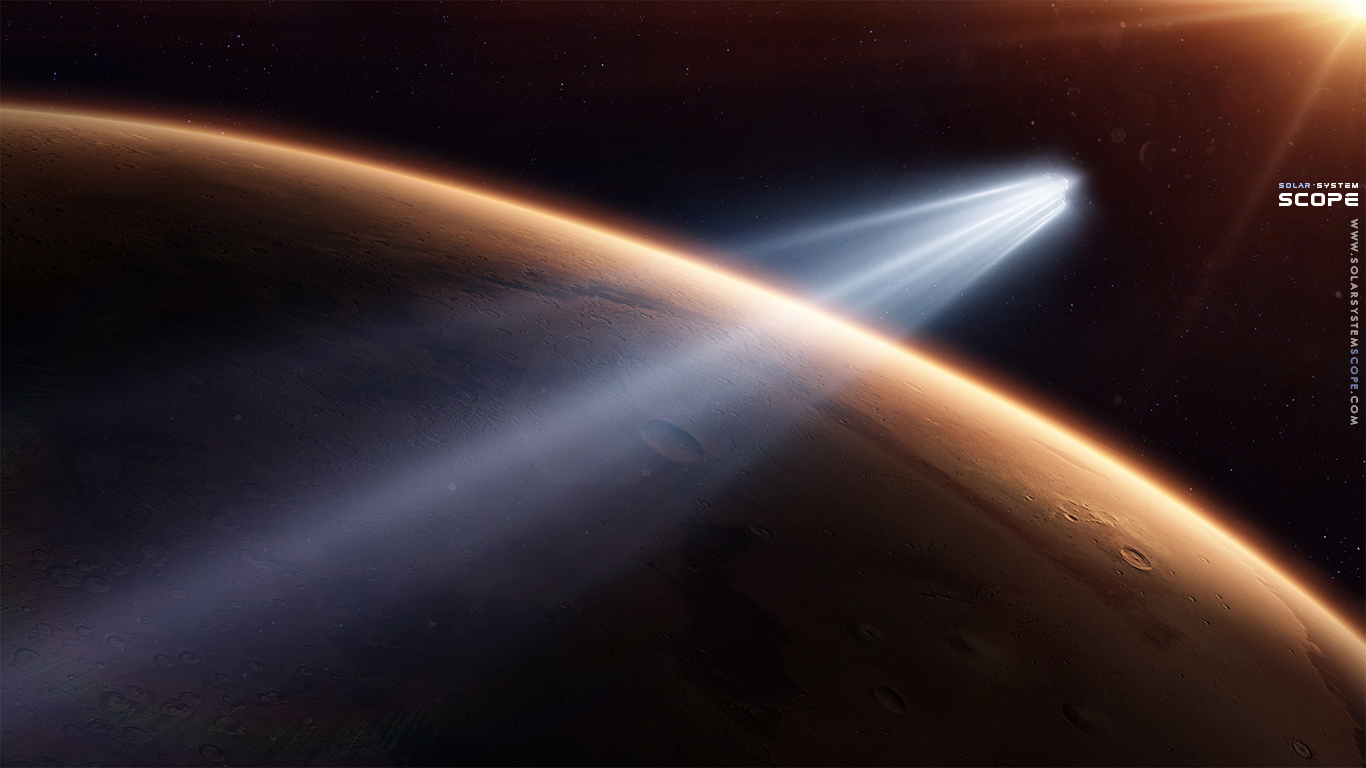
\includegraphics[height=\paperheight, keepaspectratio]{images/arive_at_target}}%
\begin{frame}
\end{frame}
\begin{frame}[t]{Sphere of Influence}
    \begin{block}{}
    Sphere of Influence(SOI) is the region around a planet in which the gravitational pull from the planet is larger
    any other.
    \begin{itemize}
        \item We are in the SOI of our sun
        \item The moon is also influenced by the gravity of the sun, but it's close enough to earth to makes its
            influence higher. So the moon is within the SOI of earth.
    \end{itemize}
    \end{block}
\end{frame}
\begin{frame}[t]{Intercept}
    \begin{block}{}
        When we are within the SOI of the target planet we need to slow down to be captured by the planet.
        \begin{itemize}
            \item Burn retrograde to slow down
            \item Keep slowing down until you fall into an highly elliptical orbit
            \item Wait for lowest point of orbit
        \end{itemize}
    \end{block}
\end{frame}
\begin{frame}[t]{Intercept}
    \begin{block}{Aerobreaking}
        Instead of having to circularize your orbit (which is expensive) we can make use of the body's atmosphere to
        slow down.
        \begin{itemize}
            \item Drop orbit just inside of the atmosphere
            \item Not too deep because you can burn up, not too shallow because it would take a very long time
            \item Wait a couple of orbits: you get closer every orbit because atmospheric drag slows you down
        \end{itemize}
    \end{block}
\end{frame}
}
\begin{frame}[t]{}
    \begin{block}{Aerobraking}
        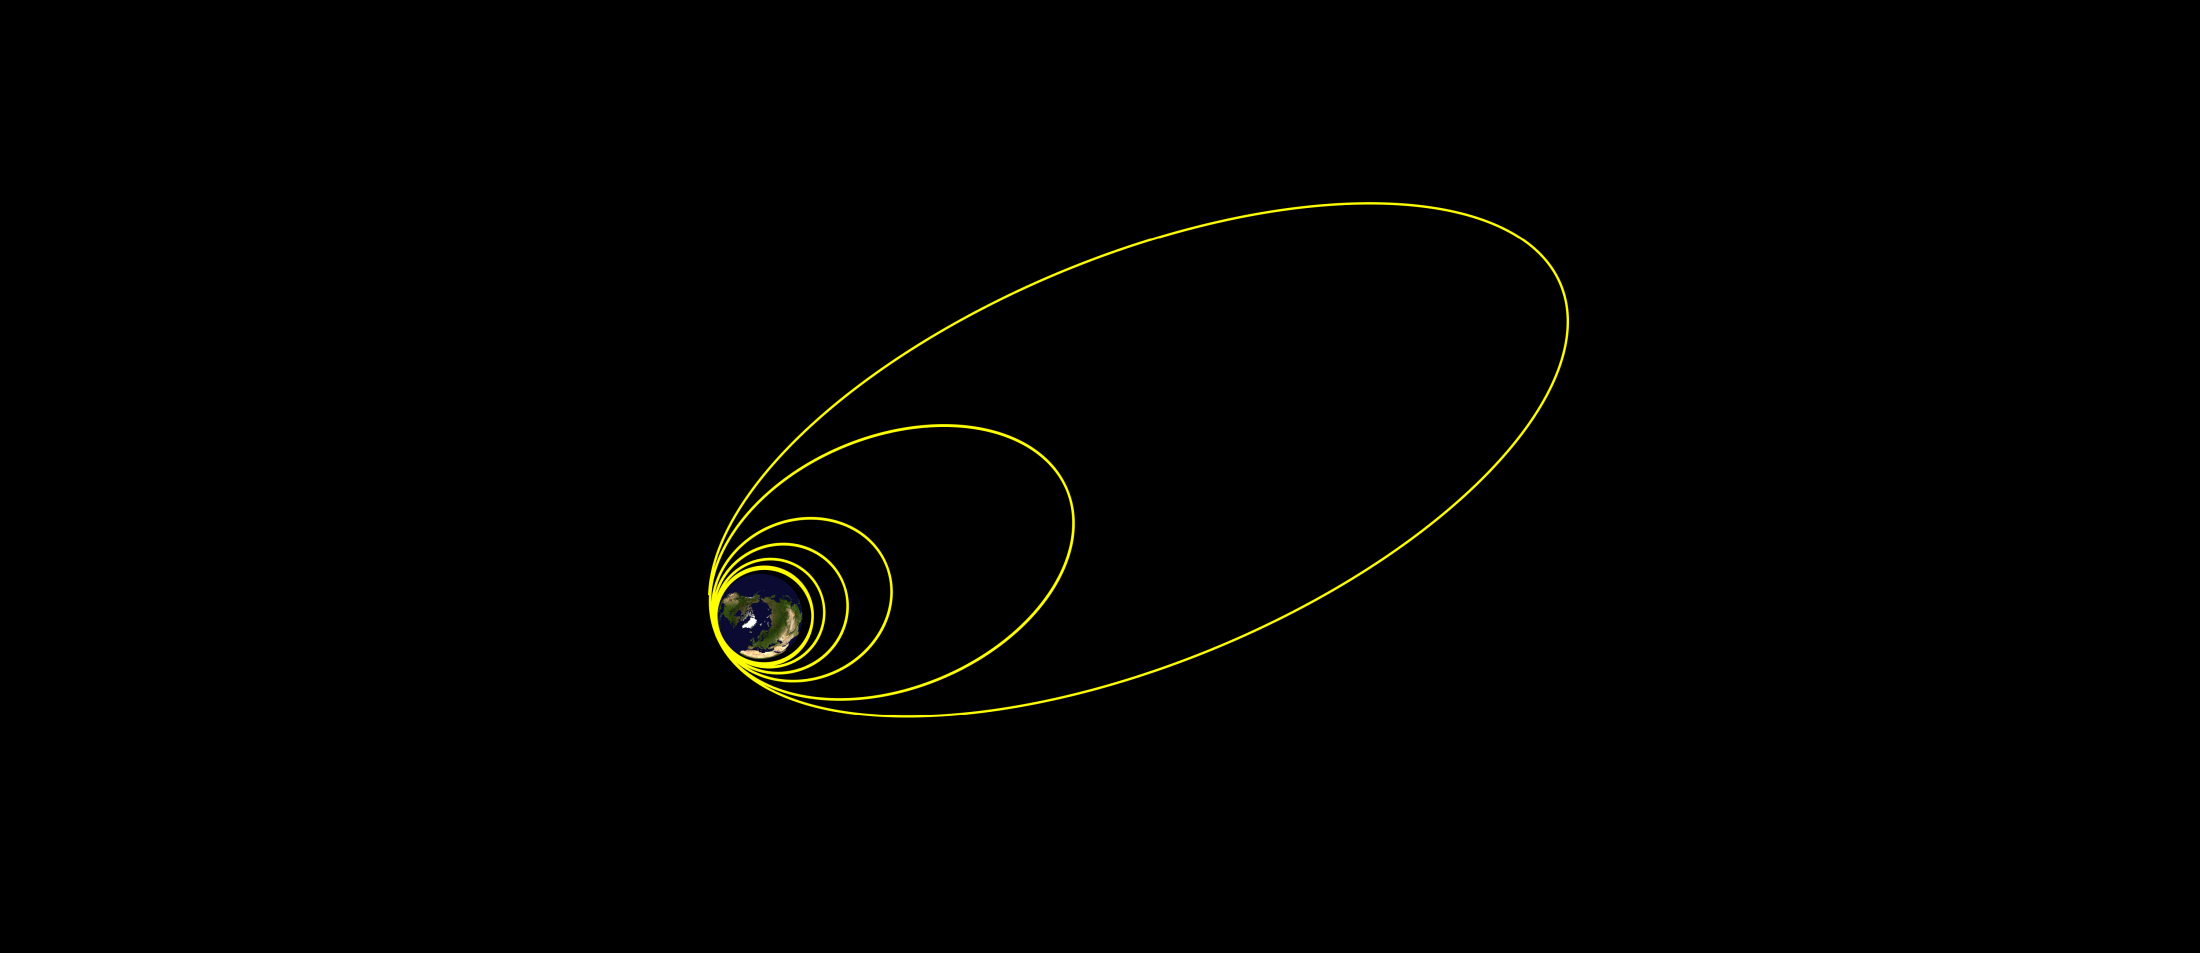
\includegraphics[width=\textwidth]{images/aerobraking}
    \end{block}
\end{frame}
